\chapter{Implementácia}
\label{chap:implementacia}
Táto kapitola pojednáva o samotnej programovej realizácií a približuje implementačné detaily tejto diplomovej práce. Kapitola vychádza z informácií uvedených v predchádzajúcich kapitolách, presnejšie popisuje prevod návrhov vykonaných v kapitole \ref{chap:analyza-navrh-riesenia} na konkrétne programové riešenie, pri ktorom boli použité technológie popísané v kapitole \ref{chap:pouzite-techologie}.  Rovnako, ako aj kapitola o analýze a návrhu riešenia, tak aj táto kapitola je rozdelená do niekoľkých logických celkov. Najprv je popísaná implementácia klientskej, či už mobilnej, alebo desktopovej aplikácie. V poradí druhou časťou je popis finálnej formy databáze, ktorá je ihneď nasledovaná popisom implementácie serverového aplikačného rozhrania, pod ktoré  spadá aj práca so snímkami. Celá kapitola je na záver ukončená popisom vybraných významnejších implementančných detailov ako je napríklad prihlasovanie, získavanie snímkov, alebo generovanie PDF súborov.

%%%%%%%%%%%%%%%%%%%%%%%%%%%%%%%%%%%%%%%%%%%%%%%%%%%%%%%%%%%%%%
\section{Implementácia klientskej aplikácie}
Aplikácia, ako sa píše už v kapitole \ref{chap:pouzite-techologie}, je implementovaná pomocou rámca pre vývoj hybridných mobilných aplikácií menom Ionic. Funkčnosť na mobilnom zariadení so systémom Android zabezpečuje rámec Cordova a na desktopovom zariadení so systémom Windows zase rámec Electron.

\subsection{Štruktúra aplikácie a popis jej komponentov}
Celá aplikácia je umiestnená v zložke \textit{src} a pozostáva z niekoľkých typov tried. Každý typ triedy je umiestnený vo vlastnom priečinku, ktorý je pomenovaný podľa tohoto typu. Konkrétne sa jedná o priečinok \textit{app}, \textit{effects}, \textit{enum}, \textit{model}, \textit{pages}, \textit{providers} a priečinok \textit{reducers}. Okrem týchto typov priečinok \textit{src} obsahuje ešte konfiguračné súbory spolu so zložkou \textit{assets} a \textit{theme}. Priečinok \textit{assets} obsahuje všetky statické súbory, ktoré sa netranspilujú (proces prekladu zdrojového kódu daného jazyka na zdrojový kód iného jazyka, v tomto prípade z Typescriptu na Javascript), konkrétne sa jedná o ikonu aplikácie spolu s obrázkom tlačidla na prihlasovanie Google účtom. Priečinok \textit{theme} obsahuje súbory, poprípade iba jeden súbor, ktorý predstavuje globálnu tému aplikácie, ktorá v sebe drží definície farieb, definície štýlov písma a iné podobné nastavenia globálneho charakteru.

V zložke \textit{app} sa nachádza hlavná komponenta a modul, ktorý predstavujú celú aplikáciu. V \textit{app} module sa nachádzajú všetky definície používaných stránok, poskytovateľov služieb, reduktorov, efektov, modálnych okien a poprípade, ak by sa v tejto práci využívali, aj direktív a rúr. Každá komponenta, a nie je tomu inak ani pri \textit{app} komponente, sa skladá vždy z troch hlavných typov súborov. Z typescript súboru, z html súboru a z scss súboru. 
\begin{itemize}
\item Typescript súbor predstavuje akýsi kontrolér danej komponenty poprípade jej logiku. 
\item Html súbor predstavuje pohľad a obsahuje zobrazované dáta jednosmerne, alebo obojsmerne naviazané na dáta v typescript súbore. 
\item Scss súbor definuje vzhľad zobrazovaného html dokumentu, avšak aplikácia v tejto práce si vystačí s bežnými komponentami Ionic rámca a tento súbor je preto často prázdny.
\end{itemize}
\textit{App} komponenta je špeciálna tým, že je globálna a existuje po celú dobu aplikácie a
preto obsahuje hlavné menu a udalosti a funkcie viazané hlavne k tomuto hlavnému menu. Vďaka tomuto menu je možné prechádzať medzi stránkami aplikácie, alebo sa odhlasovať.

V priečinku \textit{models} sa nachádzajú modely, alebo konkrétne rozhrania, všetkých hlavných entít použitých v tejto práci, menovite to sú \textit{scale.model}, \textit{therapy.model}, \textit{user.model} a \textit{wound.model}. Tieto rozhrania zabezpečujú typovú kontrolu daných entít a okrem toho behom vývoja aplikácie zabezpečovali inteligentné našeptávanie. Mimo samotných modelov, sa v tomto priečinku nachádza ešte súbor \textit{app.state}, ktorý predstavuje hlavný stav aplikácie a taktiež môže byť chápaný, ako akýsi model. \textit{App.state} slúži pre prácu s \textit{ngrx storom}, jeho efektmi a reduktormi. Celý stav aplikácie je vďaka nemu rozdelený na niekoľko podstavov určitého typu podľa vlastností tohoto \textit{app.state modelu}. Ide napríklad o typ \textit{therapy}, \textit{wound}, alebo iný a je vďaka tomu umožnené pracovať iba s vybranou časťou celkového stavu aplikácie.

V priečinku \textit{enums} sa zase nachádzajú všetky vymenúvacie typy, poprípade konštanty, ktoré sa v rámci aplikácie nemenia a sú tu definované nemenne, napevno. Ide napríklad o typy mierok, alebo stavy liečenia.

Priečinok \textit{reducers} obsahuje reduktory, ktoré slúžia na manipuláciu so stavom aplikácie. Stav aplikácie je vlastne nemenná dátová štruktúra. Stav aplikácie sa teda nemodifikuje, ale nahrádza sa vždy novým stavom. Na zmenu stavu, alebo presnejšie povedané jeho nahradenie, slúžia akcie, ktoré presne popisujú a definujú, ako sa daný stav zmení. Tieto zložky dohromady tvoria \textit{ngrx store}. Ngrx store je vlastne kontajner, alebo menežment stavu aplikácie založený na RxJS určený pre Angular a je inšpirovaný stále viac populárnym Redux. Hlavnou myšlienkou je umožnenie vytvárania komponentov schopných používať stratégiu detekcie zmeny nazvanú \textit{OnPush}. Komponenty teda načúvajú zmene stavu aplikácie, alebo jeho časti a následne na to reagujú. Všetky súbory reduktorov v sebe obsahujú okrem funkcie na zmenu stavu aj definíciu spomínaných akcií. Stav tejto aplikácie sa skladá, ako už bolo niekoľko krát spomenuté, z niekoľkých častí. Konkrétne sa jedná o časť zoznamu mierok, zoznamu liečení, zoznamu rán a o časť jednotlivej terapie a jednotlivej rany. Veľkou výhodou takéhoto prístupu je, že stačí odoslať konkrétnu akciu na \textit{ngrx store} a zmenené dáta automaticky dostanú všetky komponenty, ktoré čakajú na zmenu danej časti stavu. Tento prístup sa ukázal ako veľmi vyhovujúci, nakoľko aj pri nie až tak rozsiahlej aplikácií, ako je aplikácia tejto práce, vznikalo početné množstvo závislostí, kedy zmena dát na nejakom mieste  vyžadovala ešte aj zmenu dát na niekoľkých iných miestach.

Efekty, ktoré sú umiestnené v rovnomennej zložke \textit{effects} sú taktiež súčasťou \textit{ngrx store}. Jedná sa vlastne o akési vedľajšie účinky odoslania akcie, kedy sa nemení stav aplikácie, ale pred zmenou stavu aplikácie sa odošle ešte napríklad požiadavka na aplikačný server a získajú sa dáta. Dokončenie tejto akcie vyvolá zmenu stavu, veľmi často zmenu stavu pomocou už získaných dát zo serveru. Obrázok \ref{fig:ngrx} popisuje konkrétny prípad chovania v aplikácií, kedy sa vyvolá akcia \textit{GET\_REQUEST}. Túto akciu zachytí ako reduktor, tak aj efekt. Reduktor na akciu zareaguje tak, že iba vráti rovnakú kópiu stavu. Avšak efekt na akciu zareaguje tak, že sa vykoná požiadavka na aplikačný server a podľa úspechu/neúspechu operácie sa vyvolá akcia \textit{GET\_SUCCESS}/\textit{GET\_REQUEST} s dátami a tento nový stav je potom uložený do \textit{ngrx store}. \textit{Ngrx store} nakoniec tento stav vráti nejakej načúvajúcej komponente/komponentám. 
\begin{figure}[h]
  \centering
  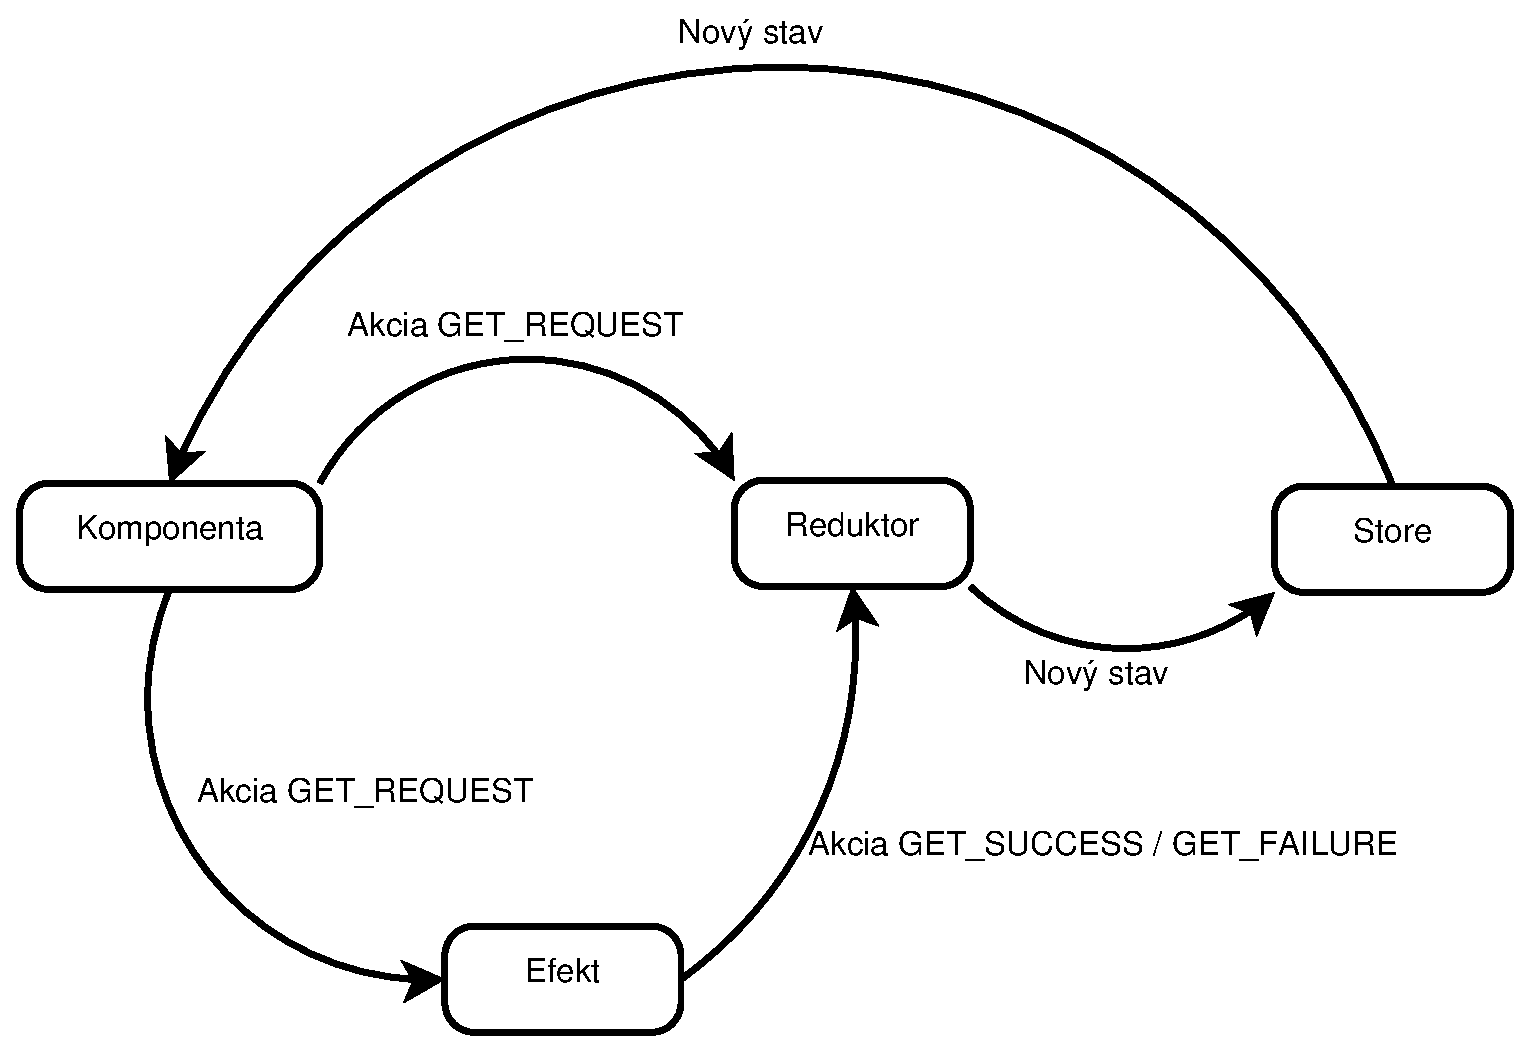
\includegraphics[scale=0.4]{fig/ngrx-efekt.eps}
  \caption{Tok dát aplikácie využívajúcej ngrx store}
  \label{fig:ngrx}
\end{figure}

Poskytovatelia nachádzajúci sa v priečinku \textit{providers slúžia}, ako názov napovedá na poskytovanie dát, či už nemenne uvedených v triede, alebo získaných z aplikačného serveru. Okrem získavania dát môžu obsahovať funkcie používané v rôznych častiach aplikácie a tak odprosťovať od písania opakovaných úsekov kódu. Jedná sa spravidla o triedy návrhového vzoru singleton, teda vzoru, ktorý sa v rámci aplikácie nachádza iba raz a inštancie týchto tried sú držané v \textit{dependency injection} kontajnere aby k nim mohli pristupovať komponenty a tak využívať ich funkcionalitu a dáta. V tejto aplikácií sa využíva celkom 5 poskytovateľov. 
\begin{itemize}
\item Api poskytovateľ (\textit{api.provider}) slúži na komunikáciu medzi aplikáciou a aplikačným serverom. Obsahuje metódy na vytváranie, mazanie a získavanie zdrojov serveru podľa daných parametrov. 
\item Auth poskytovateľ (\textit{auth.provider}) slúži na autentifikáciu a operácie k tomu príbuzné. Konkrétne obsahuje metódy na prihlasovanie, zaregistrovanie, odhlasovanie, zistenie stavu prihlásenia a taktiež drží informácie o aktuálne prihlásenom užívateľovi. 
\item Poskytovateľ dočasných náhradných dát (\textit{mock-data.provider}) slúžil počas vývoja na poskytovanie predpripravených dát pre rýchlejší vývoj, kedy sa pracovalo s týmito konštantnými dátami namiesto reálnych dát. 
\item Poskytovateľ elementov užívateľského prostredia (\textit{ui-elements.provider}) zapúzdruje niektoré často používané funkcie samotného Ionic rámca. Ide napríklad o vytváranie a zobrazovanie grafických užívateľských elementov nazvaných \textit{Toast}, alebo \textit{Alert}. Funkcie tohoto poskytovateľa takto obsahujú funkcie rámca a presnejšie špecifikujú chovanie týchto funkcií pomocou parametrov. 
\item Poskytovateľ všeobecných funkcií je posledným poskytovateľom. Tento poskytovateľ obsahuje funkcie, ktoré neboli zaradené do žiadneho iného poskytovateľa. Konkrétne tento poskytovateľ obsahuje iba 2 funkcie, a to funkciu na odstránenie vlastnosti \textit{id} a mapovanie \textit{\_id->\$oid} na \textit{id}. Funkcie sú prítomné preto, že na strane serveru a na klientskej strane sa pracuje s identifikátormi odlišne. Je to paradoxne pre jednoduchšiu prácu na klientovi, pretože databáza pracuje so svojou špecifickou štruktúrou identifikátorov a tá na klientskej strane nebola potrebná.
\end{itemize}

Posledným a zároveň aj najdôležitejším, najbohatším priečinkom na informácie a funkcionalitu je priečinok \textit{pages}. Tento priečinok obsahuje všetky stránky, obrazovky aplikácie. V koreni adresára sa nachádzajú vždy priečinky hlavných stránok. V týchto priečinkoch sa nachádzajú potom okrem samotných zdrojových súborov stránok ešte aj ďalšie stránky, alebo komponenty, ktoré súvisia s danou nadradenou stránkou sa sú v nej v podstate vnorené. Takýmto príkladom môže byť modálne okno, ktoré síce vyzerá ako stránka, ale je to vo svojej podstate súčasť inej stránky. Každá stránka, ako už bolo spomenuté pri \textit{app} module, sa skladá z niekoľkých súborov. Z typescript súboru plniaceho funkciu kontroléru. Z scss súboru, ktorý definuje výzor danej stránky a je v aplikácií v podstate skoro nepoužívaný, keďže sa používajú zväčša neupravené Ionic komponenty už v úhľadnej Material design forme. Z html súboru, ktorý predstavuje pohľad na dáta z kontroléru a definuje štruktúru stránky. A nakoniec z modulu, ktorý je prítomný iba aby bolo možné prepojiť stránky s hlavným \textit{app} modulom. Samotná aplikácia obsahuje 6 hlavných stránok. Ide o stránku obsahujúcu informácie o aplikácií (\textit{About}), stránku slúžiacu na prihlásenie (\textit{Login}), stránku obsahujúcu nastavenie a vytváranie mierok (\textit{Settings}), stránku obsahujúcu zoznam liečení (\textit{Therapy list}), stránku zobrazujúcu detail liečenia (\textit{Therapy detail}) a nakoniec stránku obsahujúcu detail rany, samotnú konkrétne zachytenú snímku (\textit{Wounbd detail}). Štruktúru členenia stránok je možné vidieť na obrázku \ref{fig:pages}.
\begin{figure}[h]
  \centering
  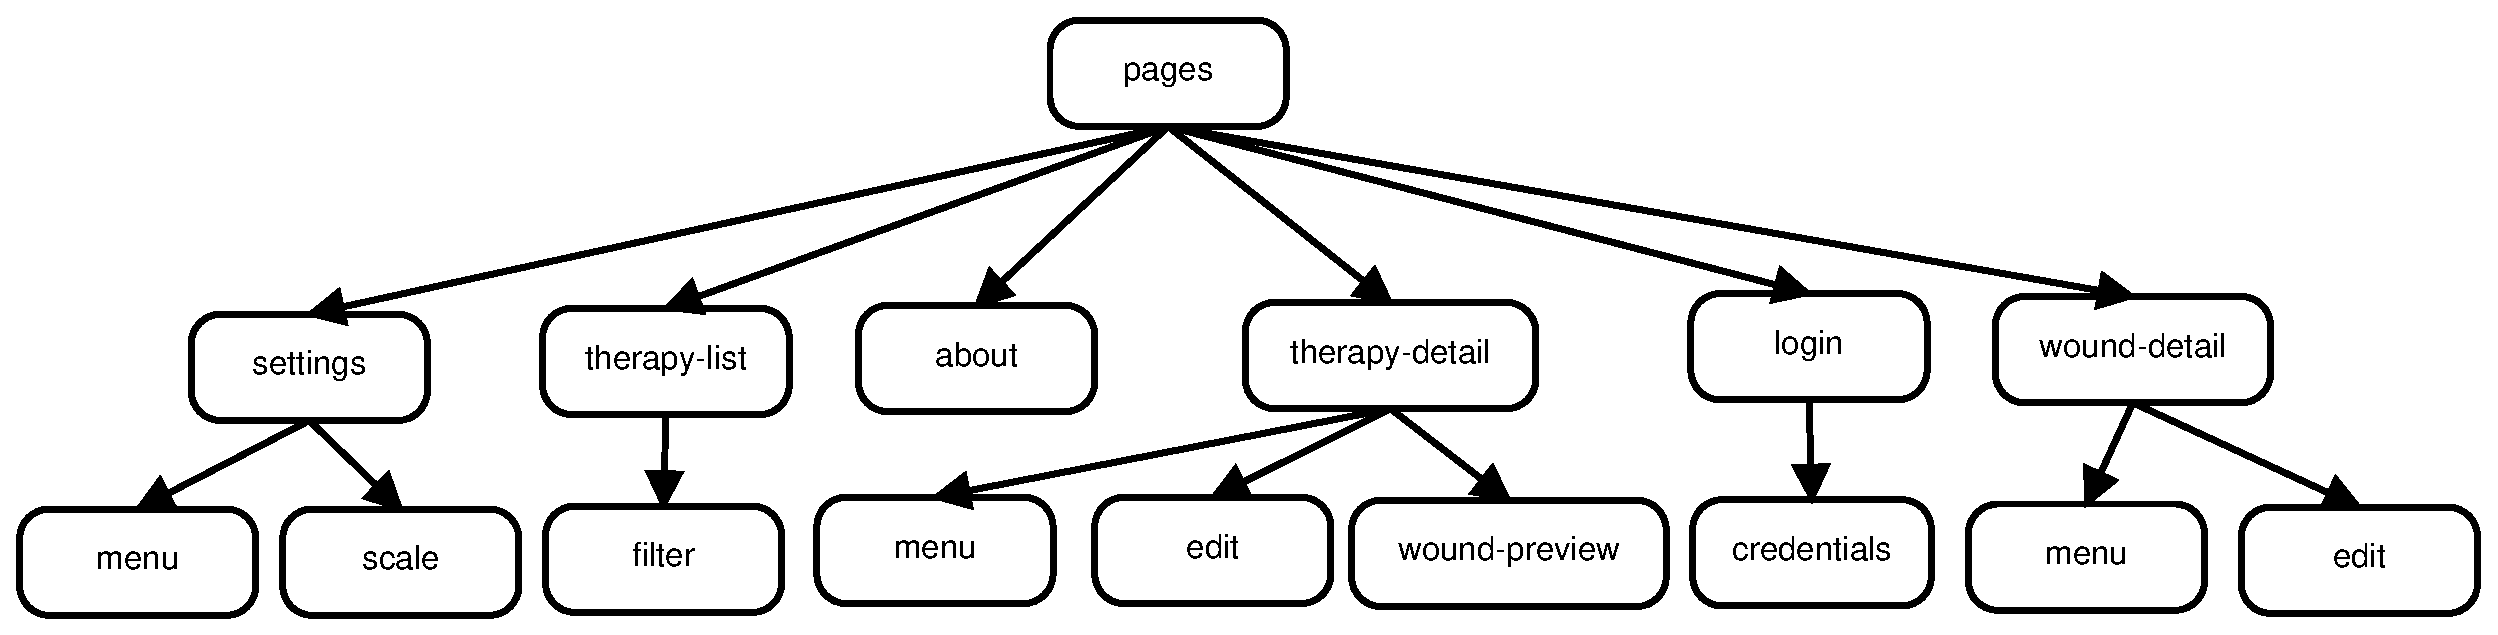
\includegraphics[scale=0.364]{fig/pages.eps}
  \caption{Štruktúra členenia stránok a ich komponentov}
  \label{fig:pages}
\end{figure}

Z obrázka je teda jasne vidieť, aké komponenty a stránky obsahujú hlavné stránky. Je zreteľne vidieť, že väčšina stránok obsahuje komponentu \textit{menu}, poprípade \textit{filter}, ako to je pri stránke zoznamu liečení, čo je vlastne kontextové menu umiestnené v pravom hornom rohu hlavičky aplikácie. Okrem komponenty \textit{menu} väčšina stránok tiež obsahuje podstránku \textit{edit}. Táto podstránka je vlastne modálne okno slúžiace na vytváranie, poprípade editovanie daného vybraného zdroja. Implementované stránky je možné vidieť na obrázkoch \ref{fig:app1} až \ref{fig:app4}.
 \begin{figure}[h]
   \begin{minipage}{0.48\textwidth}
     \centering
     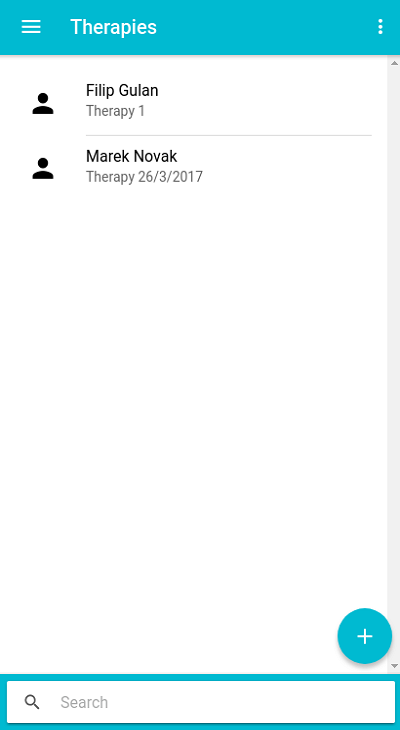
\includegraphics[scale=0.60]{fig/app1.png}
      \caption{Obrazovka zoznamu liečení}
      \label{fig:app1}
   \end{minipage}\hfill
   \begin{minipage}{0.48\textwidth}
     \centering
     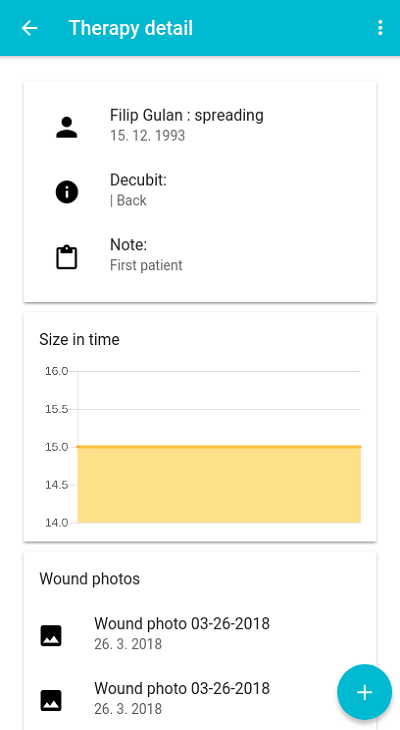
\includegraphics[scale=0.60]{fig/app2.png}
      \caption{Obrazovka detailu liečenia}
      \label{fig:app2}
   \end{minipage}
\end{figure}
\begin{figure}[h]
   \begin{minipage}{0.48\textwidth}
     \centering
     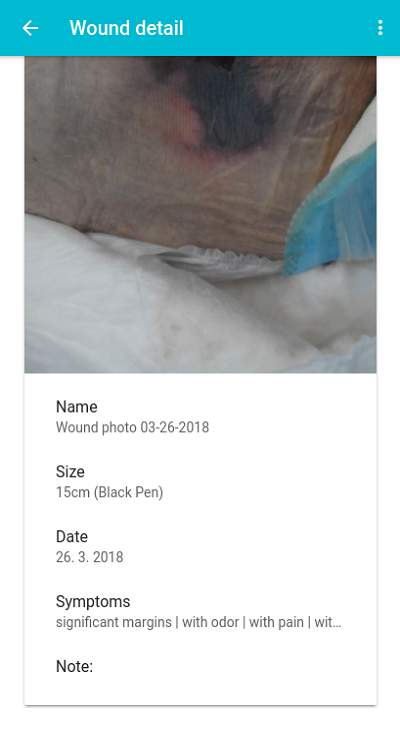
\includegraphics[scale=0.60]{fig/app3.png}
      \caption{Obrazovka detailu rany}
      \label{fig:app3}
   \end{minipage}\hfill
   \begin{minipage}{0.48\textwidth}
     \centering
     
\includegraphics[scale=0.60]{fig/app4.png}
      \caption{Obrazovka nastavení, zoznamu mierok}
      \label{fig:app4}
   \end{minipage}
\end{figure}
\newpage

\subsection{Implementačné detaily aplikácie}
Klientská aplikácia obsahuje niekoľko prvkov, ktoré stoja za zmienku a ktoré sú z hľadiska realizácie riešenia zaujímavé. Ide o nasledujúce implementačné detaily:

\begin{itemize}
\item \textbf{Filtrovanie -} Filtrovanie sa nachádza v zozname liečení. Zoznam štádií liečenia, podľa ktorých je možné filtrovať je implementovaný ako samostatná komponenta \textit{Therapy Filter} typu tzv. \textit{PopOver}, ktorá je dostupná ako kontextové menu  v pravom hornom rohu stránky. Toto menu je tvorené v rodičovskej komponente, teda v zozname liečení. V tejto rodičovskej komponente sa tiež načúva na udalosť zavretia tejto komponenty, ktorá pri svojom uzavretí vracia dané vybrané štádium. Zavretie komponenty nastáva pri výbere možnosti z filtra užívateľom. Po získaní daného štádia z komponenty sa následne nad originálnym poľom dát použije metóda \textit{filter()}, ktorá porovnáva štádia jednotlivých prvkov s užívateľom vybraným štádiom a tak užívateľ na výstup dostáva iba prvky, ktoré splňujú podmienky filtru.
\item \textbf{Vyhľadávanie -} Vyhľadávanie sa znovu nachádza na stránke zoznamu liečení, tak ako filtrovanie, a je umiestnené dole v pätičke stránky. V podstate sa jedná iba o jednoduché textové pole, ktoré je nastavené na odchytávanie zmeny svojej hodnoty a pri každej takej udalosti sa vykoná filtrovanie pomocou metódy \textit{filter()} nad originálnym poľom dát.  Konkrétne sa odfiltrovávajú položky, ktoré vo svojom názve, v krstnom mene pacienta a priezvisku pacienta neobsahujú podreťazec z vyhľadávacieho pola.
\item \textbf{Graf -} Jediné grafy, ktoré sa v aplikácií nachádzajú sú grafy zobrazované v rámci stránky detailu liečenia. Na vykresľovanie grafov bola zvolená knižnica \textit{Chart.js}, ktorá je veľmi jednoduchá na použitie, dostatočne minimalistická a pritom obsahuje všetko čo sa od knižnice takéhoto typu očakáva. Dokáže vytvoriť 6 najbežnejších typov grafov, ktoré vykresľuje na plátno (značka \textit{canvas}) a všetky takéto grafy sú plne responzívne, čo účel práce vyžaduje, keďže aplikácia je určená pre mobilné a aj desktopové zariadenia. Po tom, ako sú dáta získané z aplikačného servera, sa volá metóda \textit{createGraph()}, ktorá vykoná vyžadované nastavenia grafu a naplní graf získanými dátami. Keďže sa nejedná o knižnicu originálne vyvinutú pre Angular, alebo Ionic a pracuje s natívnym elementom, tak musel byť element plátna v html sprístupnený pre Ionic komponentu pomocou dekorátoru \textit{ViewChild}.
\end{itemize}

%%%%%%%%%%%%%%%%%%%%%%%%%%%%%%%%%%%%%%%%%%%%%%%%%%%%%%%%%%%%%%
\section{Finálna forma databáze}
Dátový model databáze predstavený v rámci jej návrhu bol v priebehu programovej realizácie upravený a prispôsobený tak, aby mohol byť uložený v NoSQL databáze akou je MongoDB. 

Prihlasovanie do aplikácie sa deje pomocou Firebase Authentification, keďže požiadavky aplikácie vyžadovali prihlásenie pomocou Google účtu a súčasne táto metóda prihlasovania je preferovaná a rozšírená v aplikáciách bežiacich na operačnom systéme Android. Z tohoto dôvodu sú dáta uložené nielen vo vlastnenej databáze, ale niektoré typy dát boli distribuované do Firebase Authentification úložiska. Táto vzdialená databáza drží práve dáta patriace k zdravotným sestrám, ošetrovateľom, doktorom, alebo jednoducho vo všeobecnosti všetkým užívateľom aplikácie.

Na obrázku \ref{fig:firebase} je možné vidieť takýto záznam jedného užívateľa vo Firebase Authentification úložisku. Takýto záznam vo Firebase Authentification úložisku pozostáva z Indentifikátora, ktorý je v prípade tejto práce vždy e-mail, z poskytovateľa, ktorý môže byť momentálne buď \textit{Google}, alebo jednoducho  \textit{E-mail/Password} (v budúcnosti pripadá do úvahy  \textit{Facebook},  \textit{Twitter} a iné), dátumu vytvorenia, dátumu posledného prihlásenia do aplikácie a užívateľovho unikátneho identifikačného čísla slúžiaceho pre jednoznačnú identifikáciu v rámci aplikácie. 
\begin{figure}[h]
  \centering
  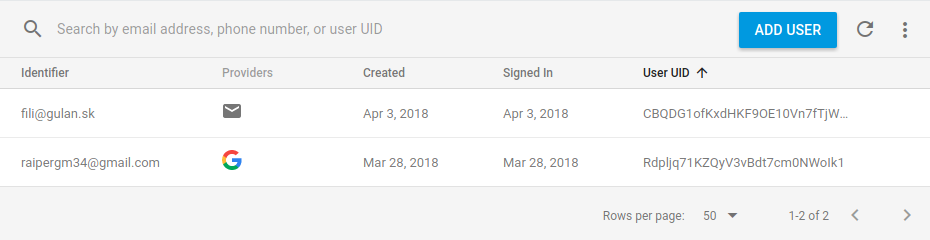
\includegraphics[scale=0.45]{fig/firebase.png}
  \caption{Ukážka záznamu vo Firebase Authentification}
  \label{fig:firebase}
\end{figure}

Liečenie, snímka rany, mierka sú potom typy dát, ktoré sú držané práve vo vlastnenom dátovom úložisku. Okrem týchto spomenutých kolekcií sa nachádza v databáze kolekcia  \textit{session}, ktorá predstavuje aktuálne sedenie užívateľa. To znamená, že táto kolekcia si drží základné informácie o aktuálne prihlásenom a v aplikácií pracujúcom užívateľovi. Dané sedenie si v sebe vždy drží token, získaný prihlásením pomocou Firebase, unikátny identifikátor užívateľa získaný znova z Firebase a ešte platformu, na ktorej je sedenie platné (buďto  \textit{core} pre internetový prehliadač,  \textit{core-electron} pre Electron desktop program, alebo  \textit{cordova-mobile-android} pre mobilnú Android aplikáciu). Výsledné kolekcie je možné vidieť v kóde.
\begin{lstlisting}[caption={Finálna štruktúra databáze},captionpos=b]
wound_database {
    scale: [
        {
            _id: 'scale-id-1',
            value: '1',
            unit: 'px',
            name: 'Scale 1',
            user: 'firebase-user-id-1',
        }
        ...
    ],
    session: [
        {
            _id: 'session-id-1',
            userId: 'firebase-user-id-1',
            platform: 'core',
        },
        ...
    ],
    therapy: [
        {
            _id: 'therapy-id-1',
            userId: 'firebase-user-id-1',
            name: 'Therapy 1',
            type: 'Decubit',
        },
        ...
    ],
    wound: [
        {
            _id: 'wound-id-1',
            therapy: 'therapy-id-1',
            user: 'firebase-user-id-1',
            originalLocation: '/home/filip/images/therapy-id-1.jpg'
            date: '154789',
            ...
        },
        ...
    ],
}
\end{lstlisting}
Kód obsahuje vždy iba pár nevyhnutných položiek, ktoré stačia na predstavu, ako je to v databáze uložené. O to, že sa v kolekcií nachádzajú ďalšie dokumenty daného typu informujú tri bodky. V tomto kóde je možné si všimnúť, ako nakoniec boli realizované vzťahy medzi jednotlivými entitami. Napríklad vzťah medzi  \textit{therapy} a  \textit{wound} je realizovaný pomocou odkazov, kedy  \textit{wound} obsahuje v sebe položku  \textit{therapy}, ktorá odkazuje na dané konkrétne liečenie podľa unikátneho identifikátoru tohoto liečenia. Vzťahy na základe referencií namiesto zanorovania štruktúr, ktoré NoSQL podporuje, boli zvolené kvôli tomu, že v podstate všetky ďalšie vzťahy sú iba vzťahy medzi entitou vo vlastnej databáze a používateľom vo Firebase Authentification úložisku a chcelo sa zachovať akýsi jednotný štandard práce s dátovými entitami.  MongoDB, ako aj iné databázy, umožňuje uložiť obrázky priamo do databáze. Pre intuitívnejšiu prácu s aplikačným serverovým rozhraním sa do databáze ale ukladajú iba cesty k súborom, ktoré sú uložené v priečinkoch na servery.

%%%%%%%%%%%%%%%%%%%%%%%%%%%%%%%%%%%%%%%%%%%%%%%%%%%%%%%%%%%%%%
\section{Implementácia serverového aplikačného rozhrania}
Aplikačné rozhranie REST nachádzajúce sa na strane serveru bolo postavené na rámci Flask a ďalších pomocných knižníc programovacieho jazyka Python. Celá programová realizácia tohoto rozhrania bola rozdelená do niekoľkých samostatných súborov a každý tento súbor predstavuje vlastne danú triedu zabezpečujúca konkrétnu sadu operácií. Realizácia obsahuje dokopy 6 súborov, z toho 1 súbor plniaci funkciu hlavnej funkcie, ktorá je mienená ako hlavný prístupový bod a 5 samostatných tried.
\begin{itemize}
\item Trieda \textit{Auth} v súbore \textit{auth.py} zabezpečuje iba jednu konkrétnu funkcionalitu a to overenie tokenu, teda či daný prichádzajúci token, ktorým sa preukazuje daný prihlásený užívateľ patrí naozaj k nejakému účtu vo Firebase Authentification.

\item Súbor \textit{database.py} obsahujúci triedu \textit{Database} zabezpečuje zase všetku prácu s MongoDB databázou za pomoci funkcií a metód knižnice pymongo. V tejto triede sa vytvára spojenie s databázou identifikovanou jej menom na danom servery a porte. V rámci tejto práce sa jedná o server s adresou \textit{127.0.0.1} teda \textit{localhost}, keďže aplikačné rozhranie a databáza sa nachádzajú na rovnakom stroji, port \textit{27017} a databázu \textit{wound\_database}. Okrem toho obsahuje metódy na prácu s dokumentami a kolekciámi tejto databáze.

\item Súbor \textit{httpStatusCode} obsahuje Hypertext Transfer Protokol stavové kódy serveru, ktoré sa využívajú pre zlepšenie čitateľnosti kódu. Sú v tejto triede uložené ako konštanty.

\item Trieda \textit{Pdf} uložená v súbore \textit{pdf.py} slúži na generovanie Portable Document Format súborov s dátami získaných z databáze. V triede sa nachádzajú 2 šablóny v HTML  formáte podľa ktorých sa generuje výsledný pdf súbor. Jedna šablóna je pre dáta o liečení a druhá pre dáta o rane. V pdf súbore liečenia sa nachádza okrem textových informácií ešte aj graf priebehu liečby, ktorý je najprv generovaný pomocou knižnice matplotlib a uložený ako obrázok. Tento obrázok sa následne vkladá do pdf suboru počas jeho tvorby. Tvorbu pdf súborov zabezpečuje knižnica pdfkit. Celý podrobný proces tvorby pdf súborov na strane serveru a prepojenie s klientskou stranou sa nachádza ďalej v kapitole.

\item Poslednou triedou, a to jednoznačne v rámci tohoto diplomového projektu aj najvýznamnejšou triedou, je trieda \textit{Vision}. Trieda je uložená znovu v rovnomennom súbore \textit{vision.py}. Zabezpečuje všetko okolo spracovania snímky rany, detekcie rany zobrazenej na snímke, detekcie mierky a vypočítania plochy rany na základe mierky a rany samotnej. Všetky tieto detekcie a výpočty sú realizované pomocou knižnice OpenCV. Spracovaniu snímky, detekcií a výpočtu plochy je ešte v tomto texte venovaný značný ďalší priestor, keďže ide o významnú časť práce.
\end{itemize}

Prístupovým bodom do aplikačného rozhrania, ktorý spracováva požiadavky klientov a následne im odpovedá je súbor \textit{main.py}. V tomto súbore sú definované všetky prístupové koncové adresy k zdrojom serveru a všetky možné metódy týchto adries. Pri požiadavke na adresu serveru bez akýchkoľvek ďalších ciest k zdroju pomocou metódy \textit{GET}  je vrátený reťazec \textit{“Wound detector API V1”}, ktorý slúži na overenie, či na danej doméne beží naimplementované aplikačné rozhranie. Pri požiadavke na adresu \textit{/static/priečinok/menosúboru} je vrátený nahraný súbor podľa svojho \textit{mena} nachádzajúci sa na servery v danom \textit{priečinku}. Adresa \textit{/auth/platforma} slúži na prihlasovanie a odhlasovanie užívateľa podľa zvolenej metódy na danej \textit{platforme}. Metódou \textit{POST} sa užívateľ do aplikácie prihlasuje, metódou \textit{DELETE} naopak odhlasuje. Ostatné adresy vo formáte \textit{/zdroj} slúžia na prístup k určenému zdroju a k manipulácií s týmto zdrojom na základe zvolenej metódy. \textit{GET} pre prístup k zdroju. \textit{POST} pre vytvorenie nového zdroju. Adresy vo formáte \textit{/zdroj/id} slúžia na prístup ku konkrétnemu zdroju identifikovanému pomocou unikátneho identifikátoru. Metódou \textit{GET} sa takýto zdroj získa, metódou \textit{PUT} modifikuje a metódou \textit{DELETE} odstráni. 


\subsection{Cross-Origin Ressource Sharing}
Odosielanie požiadaviek na server je limitované tzv. \textit{Same origin policy} a teda nie je možné prijímať odpovede na požiadavky z inej domény, ako je doména, z ktorej bolo požiadané. Túto veľmi známu limitáciu rieši \textit{Cross-origin resource sharing}, ďalej iba \textit{CORS}. CORS je vlastne mechanizmus, ktorý povoľuje zakázané zdroje na internetovej stránke, a tak aplikácie alebo internetové stránky môžu prijímať aj odpovede na požiadavky z inej domény, ako je doména, na ktorej sa aplikácia, alebo internetová stránka nachádza. Pre použitie musí nastať iba jednoduchá modifikácia hlavičiek v odpovedi serveru. Prehliadač musí posielať hlavičku \textit{Origin} nastavenú na aktuálnu doménu aplikácie, poprípade webovej stránky. Server musí posielať hlavičku \textit{Access-Control-Allow-Origin}, s hodnotou konkrétnej povolenej domény (domény aplikácie, alebo internetovej stránky), ktorá môže prijímať odpovede zo servera. Pre povolenie všetkých domén bez rozdielu sa používa *, čo je pre serverové rozhranie tejto práce chcené, keďže aplikácia bude bežať v rôznych zariadeniach a na rôznych platformách. Ďalej je možné ešte špecifikovať ďalšie nastavenia ako napríklad, ktoré \textit{HTTP} metódy budú povolené. Toto je zabezpečené hlavičkou \textit{Access-Control-Allow-Methods}, ale ani táto hlavička ani iné z rodiny \textit{Access-Control-Allow-*} nie sú v projekte využívané. 

\textit{CORS} teda funguje v nasledujúcich jednoduchých krokoch:
\begin{enumerate}
\item \textit{CORS} požiadavku iniciuje klientská strana, aplikácia.
\item Prehliadač vloží do \textit{HTTP} požiadavky hlavičky, spolu s hlavičkou \textit{Origin}.
\item Server detekuje požiadavku, vytvorí odpoveď na túto požiadavku, vloží do nej \textit{HTTP} hlavičky spolu s hlavičkou \textit{Access-Control-Allow-Origin}, ktorá indikuje, že odpoveď je povolená na danej doméne a nakoniec túto odpoveď odošle prehliadaču.
\item Prehliadač detekuje, či je odpoveď na požiadavku povolená.
    \begin{enumerate}
    \item V prípade, že je požiadavka povolená prehliadač pošle dáta ďalej aplikácií alebo internetovej stránke.
    \item V prípade neexistencie hlavičiek v odpovedi, alebo neočakávania je odpoveď zamietnutá a klientská aplikácia si nemôže prečítať tieto dáta.
    \end{enumerate}
\end{enumerate}

\begin{figure}[h]
  \centering
  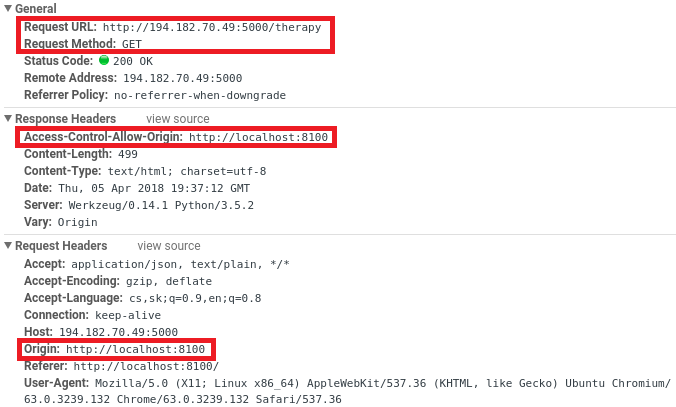
\includegraphics[scale=0.8]{fig/cors.png}
  \caption{Detail HTTP požiadavku a odpovede s hlavičkami \textit{CORS}}
  \label{fig:cors}
\end{figure}
Obrázok \ref{fig:cors} zobrazuje náhľad na požiadavku vykonanú na server a odpoveď, ktorú server vrátil. Tento obrázok bol získaný z Chrome developer tools konzole, ktorá je dostupná v internetových prehliadačoch Chrome, alebo Chromium. Na obrázku je vidieť, že sa vykonávala požiadavka na adresu \textit{http://194.182.70.49:5000/therapy} metódou \textit{GET} za účelom získania zoznamu liečení. Ďalej je možné vidieť, že do požiadavky boli vložené rôzne \textit{HTTP} hlavičky, medzi ktorými nechýba ani hlavička \textit{Origin}. Po tom, ako server spracoval požiadavku, odoslal odpoveď so štandardnými hlavičkami. Okrem štandardných hlavičiek server do odpovede vložil hlavičku \textit{Access-Control-Allow-Origin}. O povolenie mechanizmu \textit{CORS} sa v rámci tejto práce stará knižnica navrhnutá špeciálne pre Flask rámec, menom Flask-Cors.  Pre aktivovanie tejto knižnice stačí zavolať funkciu \textit{CORS(app)} a knižnica už sama do každej odpovede pridáva požadované \textit{CORS} hlavičky.

\subsection{Spracovanie snímkov}
TODO

%%%%%%%%%%%%%%%%%%%%%%%%%%%%%%%%%%%%%%%%%%%%%%%%%%%%%%%%%%%%%%
\section{Implementačné detaily}
Niektoré procesy sú vykonávané aj na strane klienta, to znamená v mobilnej, alebo desktopovej aplikácií, a aj na strane serveru v aplikačnom rozhraní. Medzi takéto procesy patrí napríklad prihlásenie užívateľa do aplikácie, získavanie snímkov, alebo generovanie PDF súborov. Všetky tieto procesy, ktoré sú vykonávané z časti na klientovi a z časti na servery sú bližšie popísané práve v tejto kapitole.

\subsection{Prihlasovanie}
Prihlasovanie v aplikácií patrí ku komplexnejším procesom v rámci programovej realizácie. Tento proces je z časti vykonávaný vo Firebase Authentification, z časti na aplikačnom serverovom rozhraní a z časti v klientskej aplikácií. Je mu z toho dôvodu venovaná samostatná kapitola obsahujúca aj dovysvetľujúci obrázok \ref{fig:login}. Firebase vo svojej momentálnej implementácií nepodporuje v Electron, v NW.js alebo v iných desktopových aplikáciach prihlasovanie pomocou Google účtu. Vo fórach a Github problémoch všetko naznačuje tomu, že v budúcnosti bude možné aj tento typ prihlasovania. Momentálne však hlavne kvôli bezpečnosti toto umožnené nie je. Tento problém bol vyriešený tak, že v desktopovej Electron aplikácií sa namiesto prihlasovania Google účtom prihlasuje iba pomocou e-mailu a hesla. Je avšak nutné upozorniť, že užívateľ zaregistrovaný a prihlásený e-mailom a heslom sa v žiadnom prípade nezhoduje s užívateľom vytvoreným a prihláseným pomocou Google účtu. Užívateľ zaregistrovaný Google účtom \textit{novak@gmail.com}, nie je ten istý užívateľ ako \textit{novak@gmail.com} zaregistrovaný e-mailom a heslom. Firebase Authentification týchto užívateľov vidí ako 2 rôznych, keďže sa jedná o 2 úplne odlišné typy prihlásenia, pričom užívateľ prihlasovaný e-mailom a heslom sa do aplikácie v podstate normálne registruje a jeho heslo neodpovedá heslu Google účtu ale heslu zvolenému pri registrácií. Na obrázku \ref{fig:electron-app} je vidieť okno desktopovej verzie aplikácie zobrazujúce prihlasovanie pomocou e-mailu a hesla.
\begin{figure}[h]
  \centering
  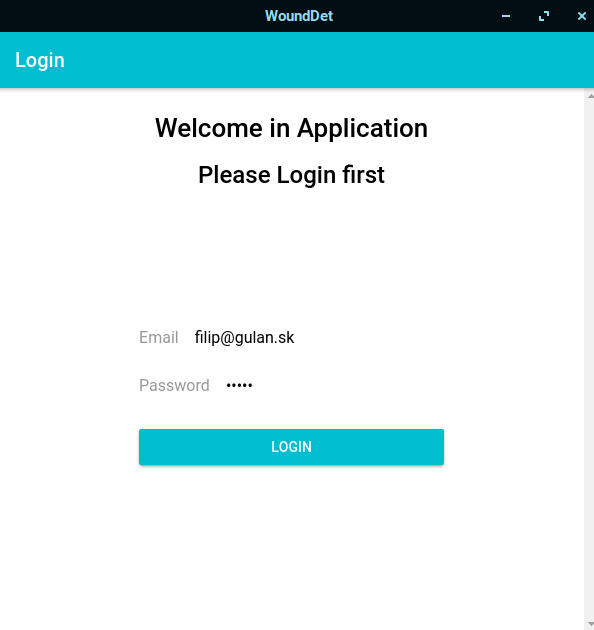
\includegraphics[scale=0.5]{fig/electron.png}
  \caption{Prihlasovacia obrazovka desktopovej verzie aplikácie}
  \label{fig:electron-app}
\end{figure}

Prihlasovanie začína na prihlasovacej obrazovke/stránke. V prípade, že sa jedná o mobilnú Android aplikáciu, prípadne internetovú aplikáciu, tak je ponúknuté prihlasovanie aj pomocou Google účtu aj pomocou e-mailu a hesla. V prípade, že sa jedná o desktopovú verziu aplikácie, tak sa tam nachádza iba formulár slúžiaci na prihlasovanie pomocou e-mailu a hesla. Ide síce o 2 v podstate odlišné metódy prihlásenia, avšak vďaka Firebase Authentification ich prihlasovací cyklus v rámci aplikácie prebieha absolútne rovnako. Jediná odlišnosť je v tom, keď sa užívateľ prihlasuje prvý krát do aplikácie pomocou Google účtu, tak Firebase vytvorí vo svojej databázy záznam automaticky. Naopak pri metóde prihlasovania pomocou e-mailu a hesla sa tento záznam musí najprv vytvoriť programovo, teda pri prvom prihlasovaní prebieha akási prvotná registrácia užívateľa, ktorú vykonáva samotná klientská aplikácia. Po stlačení tlačítka na prihlásenie Google účtom, alebo tlačítka na prihlásenia vo formulári, sa vykoná požiadavka na server Firebase Authentification, ktorá sa pokúsi užívateľa prihlásiť a v prípade úspechu vráti objekt užívateľa s ostatnými informáciami, ako je napríklad platný token. Získaný token sa následne odošle na serverové aplikačné rozhranie tejto práce na koncovú adresu \textit{/auth/platforma} metódou \textit{POST}, kde platforma predstavuje platformu zariadenia, z ktorého sa užívateľ pokúša prihlásiť. Pred vykonaním požiadavky sa ešte nastaví \textit{HTTP} hlavička \textit{Authorization} na hodnotu získaného tokena. Na servery je tento token overovaný, či sa jedná o platný token získaný z Firebase Authentification. Okrem samotného overenia je znovu získaný aj užívateľ, ktorému patrí tento token. V prípade, že je token úspešne overený, tak sa vytvorí v databázy v kolekcií \textit{session} záznam predstavujúci dané sedenie identifikované svojim unikátnym identifikátorom a obsahujúce Firebase Authentification token, unikátny identifikátor prihláseného užívateľa a platformu z ktorej prihlásenie nastalo. Po tom, ako je token overený a je vytvorený dokument kolekcie \textit{session}, tak je následne prihlásený užívateľ vrátený v odpovedi do aplikácie. Vrátený užívateľ sa následne uloží do poskytovateľa autentifikácie (\textit{auth.provider}) a tieto informácie sú zobrazené v hlavnom menu, konkrétne je zobrazené meno, priezvisko, e-mail a fotka užívateľa. Po tom, ako bol užívateľ prihlásený v obidvoch častiach, aj vo Firebase Authentification časti a aj v časti serverového aplikiačného rozhania, je možné vykonávať dotazy na server pre získanie súkromných dát, medzi ktoré patria doslova všetky požiadavky serveru, ako napríklad získanie zoznamu liečení, zoznamu rán a podobne. Všetky požiadavky po procese prihlásenia teda obsahujú \textit{HTTP} hlavičku \textit{Authorization} s hodnotou tokenu z Firebase Authentification. Po požiadaní serveru o zdroj sa na servery táto hlavička získa a porovnáva sa, či sa v databázy v kolekcií session nachádza takýto užívateľ. V prípade, že sa takýto užívateľ v kolekcií nenachádza, server vráti \textit{401 UNAUTHORIZED}. V opačnom, v kladnom prípade je užívateľ získaný z databázy a jeho identifikátor je ďalej používaný pre získavanie žiadúcich zdrojov. Celý tento proces je pre názornosť zobrazený na obrázku \ref{fig:login}. 
\begin{figure}[h]
  \centering
  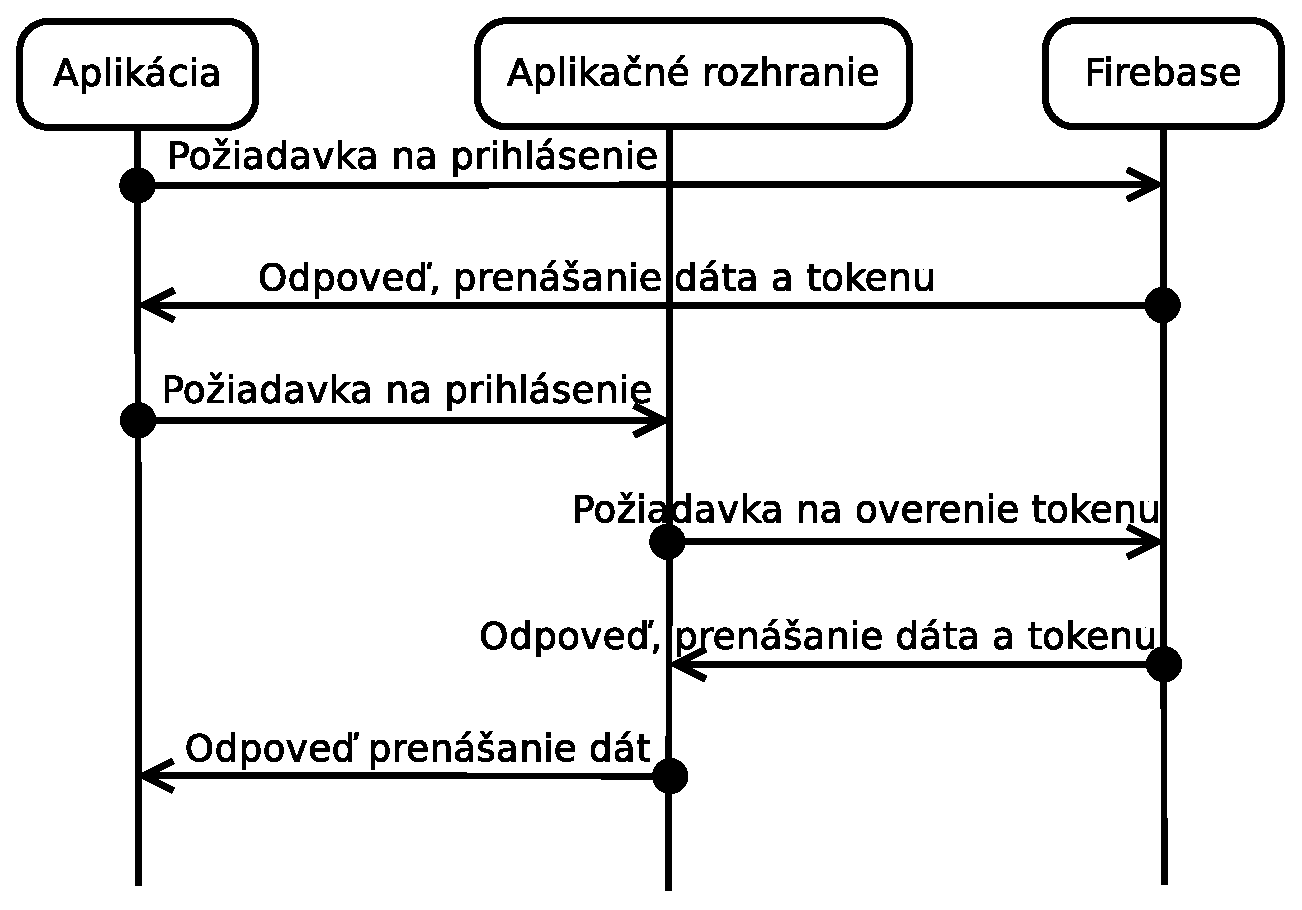
\includegraphics[scale=0.5]{fig/login.eps}
  \caption{Priebeh prihlasovania}
  \label{fig:login}
\end{figure}

\subsection{Získavanie snímkov}
Medzi najvýznamnejšie procesy práce patrí jednoznačne aj proces vyhotovovania snímkov. Tento proces prebieha z časti v aplikácií a z časti na aplikačnom servery. Proces začína na stránke detailu konkrétneho liečenia, kde si užívateľ zvolí v rozkladacom plávajúcom tlačítku, či chce použiť už hotové snímky z lokálneho úložiska svojho zariadenia, alebo chce ranu rovno zosnímať pomocou mobilnej počítačovej kamery, poprípade fotoaparátu. Ak si užívateľ vyberie prvú možnosť a zvolí si už existujúcu snímku z lokálneho úložiska, tak sa táto snímka predáva modálnemu oknu ukážky rany pomocou \textit{NavParams}. V druhom prípade sa iba prejde do rovnakého modálneho okna ale bez predania dát. V tomto modálnom okne sa v konštruktore detekuje, či boli predané nejaké dáta. V prípade existencie dát, sú tieto dáta zakódované do formátu \textit{Base64} a spôsobom, aký je bežný aj napríklad pre formulárové dáta tejto aplikácie, je obrázok odoslaný na aplikačný server. (\textit{Base64} je kódovanie, alebo mechanizmus, ktorý povoľuje prenos binárnych dát cez média, ktoré umožňujú iba prenos textu. Vznikol kvôli potrebe pridávať do e-mailov obrázkový, video alebo iný binárny obsah. Kóduje vždy 3 oktety binárnych dát pomocou 4 \textit{ASCII} znakov). V prípade, že sa dáta v do komponenty nepredali, tak sa v konštruktore aktivuje kamera a užívatel má tak možnosť zosnímať ranu priamo. Po vyhotovení sa snímka tejto rany znovu prekonvertuje do \textit{Base64} formátu a odošle na aplikačný server. Aplikačný server príjme požiadavku obsahujúcu takto zakódovaný obrázok, obrázok prekóduje naspäť do originálneho kódovania, vytvorí dočasný dokument v kolekcií \textit{wounds} a obrázok uloží do priečinku \textit{static/shoots} s menom \textit{identifikátoru} vytvoreného dočasného dokumentu v kolekcií \textit{wounds}. Tento obrázok sa následne spracuje a prebehnú všetky požadované výpočty. Po úspechu tejto operácie je v aplikácií zobrazený daný spracovaný obrázok, tak že HTML element \textit{img} obsahuje v atribúte \textit{src} hodnotu adresy, ktorá sprostredkováva obrázky uložené na servery (\textit{/static/shoots/wound-id.jpg}). Zobrazením obrázku je užívateľ vyzvaný, či sa daný obrázok použije ako finálna snímka rany, alebo chce proces opakovať a použiť, alebo vytvoriť inú snímku. V prípade nevyhovujúcej snímky, kedy napríklad bola rana nesprávne detekovaná kvôli svetelným alebo iným podmienkam, tak užívateľ zvolí možnosť opakovať proces a znovu sa aktivuje kamera, s tým že dočasný obrázok je zo serveru vymazaný. V prípad, že obrázok vyhovuje, prejde sa do modálneho okna editácie/vytvárania snímky, kde užívateľ je nútený vyplniť konečné informácie potrebné pre vytvorenie snímky. Povinnou položkou v tomto formulári je iba meno, ktoré je prednastavené na \textit{“Wound photo + aktuálny dátúm”} a položka mierky. Po vyplnení a odoslaní formulára je vytvorená konečne finálna snímka rany zobrazujúca sa v zozname snímok v detaile daného liečenia. Ak sa proces v ktoromkoľvek kroku preruší, tak je dočasný dokument z databáze spolu s dočasnou snímkou vymazaný.

\subsection{Generovanie PDF súborov}
Ďalším procesom, ktorý presahuje rozdelenie na proces aplikácie a proces serveru je generovanie súborov typu Portable Document Format s informáciami o danom liečení, alebo o danej konkrétnej rane. Generovanie je možné zahájiť na stránke detailu liečenia v kontextovom menu, alebo v kontextovom  menu na stránke detailu rany. Napriek tomu, že Javascript knižnice dokážu programovo vytvárať jednoduché PDF súbory, bola zvolená možnosť generovania týchto súborov na servery. Rozhodnutie bolo vykonané hlavne kvôli obmedzeniam vo finálnej Android aplikácií, kde aj po početných pokusoch sa nepodarilo takto generovaný súbor správne uložiť do zariadenia. PDF súbory sa teda generujú na servery. Proces generovania súboru iniciuje klientská aplikácia, alebo lepšie povedané užívateľ výberom možnosti generácie PDF v kontextovom menu. Po výbere tejto možnosti je úžívateľovi zobrazené okno načítania, ktoré je prítomné po celú dobu, až pokiaľ nie je súbor definitívne stiahnutý, alebo nenastala nejaká neočakávaná chyba. Následne je odoslaná na server požiadavka o generovanie súboru \textit{HTTP} metódou \textit{POST}. Server túto požiadavku príjme, získa informácie z databáze potrebné pre PDF súbor a pomocou knižnice PDFKit začne podľa HTML šablóny generovať samotný PDF súbor, ktorý uloží do priečinku \textit{static/pdfs}. V prípade, že PDF súbor má obsahovať aj graf, konkrétne PDF súbory liečení obsahujú grafy, tak sa najprv tento graf vygeneruje a uloží sa ako Portable Network Graphic obrázok do priečinku \textit{static/temp} odkiaľ sa potom použije v šablóne.  Po skončení operácie na servery je klientovi vrátený \textit{HTTP} statu kód \textit{200}. Týmto status kódom užívateľ vie, že PDF súbor je pripravený na stiahnutie. Sťahovanie samotného PDF súboru prebieha rozdielne pri Mobilnej a Desktopovej aplikácií. Pre stiahnutie súboru na platforme Android sa využíva natívny Cordova pluginu menom FileTransfer, ktorý súbor zo serveru stiahne a uloží do externého dátového priečinku, to je do priečinku \textit{Android/data/net.raiper34.wounddetector/files}. Užívateľ je o tomto úspechu informovaný pomocou upozorňovacieho okna, v ktorom je zobrazená cesta k súboru. Aj v prípade  desktopovej verzie nebolo možné stiahnuť súbor iba pomocou tradičných metód, ako napríklad pridanie atribútu \textit{download} pre kotvový element. Namiesto toho sa musela vykonať požiadavka na server metódou \textit{GET} a špecifikovať hlavička \textit{responseType} nastavená na hodnotu \textit{arrayBuffer}. Dáta, ktoré boli následne získané zo serveru sa potom pomocou  objektu \textit{Blob} a knižnice FileSaver uložili na užívateľom vybrané miesto. Keďže užívatel si sám volí, kde sa súbor uloží, tak o úspechu je informovaný obyčajnou \textit{Toast} komponentou so základnou hláškou úspechu.